\documentclass[polish,a4paper]{article}
\usepackage{lmodern}
\usepackage{amssymb,amsmath}
\usepackage{ifxetex,ifluatex}
\usepackage{fixltx2e} % provides \textsubscript
\ifnum 0\ifxetex 1\fi\ifluatex 1\fi=0 % if pdftex
  \usepackage[T1]{fontenc}
  \usepackage[utf8]{inputenc}
\else % if luatex or xelatex
  \ifxetex
    \usepackage{mathspec}
  \else
    \usepackage{fontspec}
  \fi
  \defaultfontfeatures{Ligatures=TeX,Scale=MatchLowercase}
\fi
% use upquote if available, for straight quotes in verbatim environments
\IfFileExists{upquote.sty}{\usepackage{upquote}}{}
% use microtype if available
\IfFileExists{microtype.sty}{%
\usepackage{microtype}
\UseMicrotypeSet[protrusion]{basicmath} % disable protrusion for tt fonts
}{}
\usepackage[margin=1in]{geometry}
\usepackage{hyperref}
\PassOptionsToPackage{usenames,dvipsnames}{color} % color is loaded by hyperref
\hypersetup{unicode=true,
            pdftitle={Ekspresowa analiza ryzyka:},
            pdfkeywords={Ocena Zagrożenia Agrofagiem; Helicoverpa zea},
            colorlinks=true,
            linkcolor=TealBlue,
            citecolor=TealBlue,
            urlcolor=Cerulean,
            breaklinks=true}
\urlstyle{same}  % don't use monospace font for urls
\ifnum 0\ifxetex 1\fi\ifluatex 1\fi=0 % if pdftex
  \usepackage[shorthands=off,main=polish]{babel}
\else
  \usepackage{polyglossia}
  \setmainlanguage[]{polish}
\fi
\usepackage{longtable,booktabs}
\usepackage{graphicx,grffile}
\makeatletter
\def\maxwidth{\ifdim\Gin@nat@width>\linewidth\linewidth\else\Gin@nat@width\fi}
\def\maxheight{\ifdim\Gin@nat@height>\textheight\textheight\else\Gin@nat@height\fi}
\makeatother
% Scale images if necessary, so that they will not overflow the page
% margins by default, and it is still possible to overwrite the defaults
% using explicit options in \includegraphics[width, height, ...]{}
\setkeys{Gin}{width=\maxwidth,height=\maxheight,keepaspectratio}
\IfFileExists{parskip.sty}{%
\usepackage{parskip}
}{% else
\setlength{\parindent}{0pt}
\setlength{\parskip}{6pt plus 2pt minus 1pt}
}
\setlength{\emergencystretch}{3em}  % prevent overfull lines
\providecommand{\tightlist}{%
  \setlength{\itemsep}{0pt}\setlength{\parskip}{0pt}}
\setcounter{secnumdepth}{5}
% Redefines (sub)paragraphs to behave more like sections
\ifx\paragraph\undefined\else
\let\oldparagraph\paragraph
\renewcommand{\paragraph}[1]{\oldparagraph{#1}\mbox{}}
\fi
\ifx\subparagraph\undefined\else
\let\oldsubparagraph\subparagraph
\renewcommand{\subparagraph}[1]{\oldsubparagraph{#1}\mbox{}}
\fi

%%% Use protect on footnotes to avoid problems with footnotes in titles
\let\rmarkdownfootnote\footnote%
\def\footnote{\protect\rmarkdownfootnote}

%%% delete abstract name
\renewcommand{\abstractname}{\vspace{-\baselineskip}}

%%% Change title format to be more compact
\usepackage{titling}

% Create subtitle command for use in maketitle
\newcommand{\subtitle}[1]{
  \posttitle{
    \begin{center}\large#1\end{center}
    }
}

% Create corresponding command for use in maketitle
\newcommand{\corresponding}[1]{%
   \gdef\Mail{#1}}
 \newcommand{\Mail}{}
 \renewcommand{\maketitlehookc}{%
   \par\noindent \Mail}

\newcommand*{\email}[1]{\href{mailto:#1}{\nolinkurl{#1}} }

\setlength{\droptitle}{-2em}

  \title{Ekspresowa analiza ryzyka: \textit{Helicoverpa zea} (Boddie, 1850)}
    \pretitle{\vspace{\droptitle}\centering\huge}
  \posttitle{\par}
  
  \author{Wojciech Kubasik\textsuperscript{A}, Magdalena Gawlak\textsuperscript{A}, Michał Czyż\textsuperscript{A}, Agata Olejniczak\textsuperscript{A}, Tomasz Kałuski\textsuperscript{A}}
    \preauthor{\flushleft\large\emph Autorzy: }
  \postauthor{\par A: Instytut Ochrony Roślin, ul. Węgorka 20, Poznań, 60-318}
  
\corresponding{\small Autor korespondencyjny:
     \textit{\href{mailto:plantquarantine@pra.org}{\nolinkurl{plantquarantine@pra.org}}}
  
    
    
    
    
  }

    \predate{\flushleft\large\emph  Data: }
  \postdate{\par }
    \date{Październik 11, 2017\footnote{Raport został wygenerowany w R (R Core
  Team, \protect\hyperlink{ref-rcore2018}{2018}) z użyciem knitr i
  bookdown (Xie, \protect\hyperlink{ref-xie2016}{2016},
  \protect\hyperlink{ref-xie2015}{2015})}}

%%%\corresponding()


\addto\captionspolish{%
  \renewcommand{\partname}{Etap}%
  \renewcommand{\abstractname}{}%
}
\usepackage{hyperref}
\usepackage[dvipsnames,table]{xcolor}
\usepackage{tcolorbox}
\tcbuselibrary{raster,skins}
\usepackage{tabto}
\usepackage{booktabs}
\usepackage{longtable}
\usepackage{array}
\usepackage{multirow}
\usepackage{wrapfig}
\usepackage{float}
\usepackage{colortbl}
\usepackage{pdflscape}
\usepackage{tabu}
\usepackage{threeparttable}
\usepackage{threeparttablex}
\usepackage[normalem]{ulem}
\usepackage{makecell}
\usepackage{array,tabularx}
\usepackage{colortbl}
\usepackage[backend=bibtex,citestyle=authoryear]{biblatex}
\addbibresource{pra.bib}

\begin{document}
\begin{abstract}
\begin{tcolorbox}[minipage,colback=Goldenrod,colframe=black,arc=1pt,outer arc=1pt,adjusted title= \textbf{Podsumowanie Analizy Ryzyka Zagrożenia Agrofagiem (Ekspres PRA) dla \textit{Helicoverpa zea}}]
\normalsize
\textbf{Obszar PRA:} Rzeczpospolita Polska\newline
\textbf{Opis obszaru zagrożenia:} uprawy   polowe   (głównie   kukurydzy),   przede   wszystkim   w   Polsce północno-zachodniej, w niewielkim stopniu również uprawy w warunkach chronionych w całej Polsce.\newline
\noindent\rule{\linewidth}{0.5pt}
\textbf{Główne wnioski:} \newline
\textit{H. zea} jest gatunkiem motyla z rodziny sówkowatych (Noctuidae) szeroko rozsiedlonym w cieplejszych rejonach obu Ameryk. Gąsienice żerują polifagicznie na wielu roślinach, przynosząc wysokie straty ekonomiczne, między innymi w uprawie kukurydzy, sorgo, bawełny i pomidorów. Motyle wykazują duże zdolności migracyjne i są wstanie zasiedlać czasowo miejsca o znacznie chłodniejszym klimacie (np. północ Kanady, południe Argentyny). W obecnych warunkach klimatycznych Polski powstanie osiadłych populacji \textit{H. zea}  jest bardzo mało prawdopodobne, jednak w przypadku  rozwinięcia się licznych populacji na południu Europy, terytorium naszego kraju znajdzie się w zasięgu migrujących osobników (analogiczna sytuacja ma miejsce w wypadku bliźniaczego gatunku \textit{H. armigera}). Istnieje także ryzyko, że w przypadku zawleczenia gatunek ten może wyrządzić szkody w uprawach pod osłonami – zarówno roślin ozdobnych jak i warzyw.'\newline
\textbf{Ogólna ocena ryzyka: } \tcbox[enhanced,frame style={opacity=0.25},interior style={opacity=0.5},size=tight,colframe=Bittersweet,colback=Bittersweet!70!white,shrink tight,extrude by=0.5mm,nobeforeafter,arc=2.5pt,outer arc=2.5pt]{Średnie}.\newline\newline
\noindent\rule{\linewidth}{0.5pt}
  \begin{tcolorbox}[title=\textcolor{black}{\textbf{Ryzyko fitosanitarne dla zagrożonego obszaru:} },after skip=0mm,inherit height,arc=1pt,outer arc=1pt,colframe=Dandelion,colback=Yellow]
    \begin{tcbraster}[raster columns=3,fonttitle=\bfseries,nobeforeafter,colback=Yellow,colframe=Bittersweet,arc=1pt,outer arc=1pt,boxrule=0.5pt,bottomrule=1pt,toprule=1pt,center title]
      \begin{tcolorbox}[adjusted title=Wysokie,halign=flush center]
        \textbf{.}
      \end{tcolorbox}\hfill
      \begin{tcolorbox}[adjusted title=Średnie,halign=flush center]
        \textbf{X}
      \end{tcolorbox}\hfill
      \begin{tcolorbox}[adjusted title=Niskie,halign=flush center]
        \textbf{.}
      \end{tcolorbox}
    \end{tcbraster}
  \end{tcolorbox}
  \begin{tcolorbox}[title=\textcolor{black}{\textbf{Poziom niepewności oceny:} },before skip=0pt,inherit height,arc=1pt,outer arc=1pt, colframe=Dandelion, colback=Yellow]
    \begin{tcbraster}[raster columns=3,fonttitle=\bfseries,nobeforeafter,colback=Yellow,colframe=Bittersweet,arc=1pt,outer arc=1pt,boxrule=0.5pt,bottomrule=1pt,toprule=1pt,center title]
      \begin{tcolorbox}[adjusted title=Wysoka,halign=flush center]
        \textbf{.}
      \end{tcolorbox}\hfill
      \begin{tcolorbox}[adjusted title=Średnia,halign=flush center]
        \textbf{X}
      \end{tcolorbox}\hfill
      \begin{tcolorbox}[adjusted title=Niska,halign=flush center]
        \textbf{.}
      \end{tcolorbox}
    \end{tcbraster}  
  \end{tcolorbox}
\noindent\rule{\linewidth}{0.5pt}  
\textbf{Inne rekomendacje:
\begin{itemize}
\item Należy na bieżąco sprawdzać informacje o znaczących stratach wyrządzanych przez \textit{H. armigera} i na podstawie odłowionych osobników dorosłych sprawdzać, czy nie są to przedstawiciele \textit{H. zea}.
\end{itemize}}
\end{tcolorbox}
\end{abstract}

\maketitle

\part{Wstęp}\label{part-wstep}

\textbf{Powód wykonania PRA:} \emph{Helicoverpa zea} jest gatunkiem
rozprzestrzenionym w strefach tropikalnych, subtropikalnych i
umiarkowanych obu Ameryk. Gąsienica żeruje polifagicznie na wielu
gatunkach roślin, zarówno dzikich, jak i uprawnych. W Ameryce Północnej
powoduje ona znaczne straty w uprawie, między innymi kukurydzy i soi.
Ponieważ motyle potrafią migrować na znaczne odległości, gąsienice są
spotykane również w regionach, gdzie gatunek ten nie jest w stanie
przezimować. Istnieje ryzyko zawleczenia tego gatunku do Europy, gdzie
będzie mógł się dalej rozprzestrzeniać samoistnie.

\textbf{Obszar PRA:} Rzeczpospolita Polska

\part{Ocena zagrożenia
Agrofagiem}\label{part-ocena-zagrozenia-agrofagiem}

\begin{enumerate}
\def\labelenumi{(\arabic{enumi})}
\tightlist
\item
  Taksonomia:
\end{enumerate}

\begin{itemize}
\item
  Królestwo: Animalia
\item
  Typ: Arthropoda
\item
  Podtyp: Hexapoda
\item
  Gromada: Insecta
\item
  Rząd: Lepidoptera
\item
  Rodzina: Noctuidae
\item
  Rodzaj: \emph{Helicoverpa}
\item
  Gatunek: \emph{Helicoverpa zea} (Boddie, 1850)*
\end{itemize}

Na podstawie: EPPO (\protect\hyperlink{ref-eppo2018}{2018})

\textbf{Synonimy:} \emph{Heliothis zea} (Boddie, 1850), \emph{Phalaena
zea} (Boddie, 1850), \emph{Bombyx obsoleta} Fabricius 1775,
\emph{Heliothis umbrosa} Grote

\textbf{Nazwa powszechna:} American bollworm, corn earworm, tomato
fruitworm, New World bollworm (angielska), Chenille des épis du maïs
(francuska), Amerikanischer Baumwollkapselwurm (niemiecka)

\begin{enumerate}
\def\labelenumi{(\arabic{enumi})}
\setcounter{enumi}{1}
\tightlist
\item
  Informacje ogólne o agrofagu:
\end{enumerate}

\emph{Helicoverpa zea} jest gatunkiem rozpowszechnionym na obu
kontynentach amerykańskich, o dużych skłonnościach migracyjnych.
Szczegółowe informacje o tym gatunku dostępne są na stronach (EPPO
(\protect\hyperlink{ref-eppo2018}{2018}), CABI/EPPO
(\protect\hyperlink{ref-cabieppo2017}{2017})) oraz stronach CABI
(\protect\hyperlink{ref-cabi2017}{2018}). Dużo informacji o biologii i
szkodliwości można znaleźć także na stronach University of Florida
Capinera (\protect\hyperlink{ref-capinera2000}{2000}).

Gąsienice żerują polifagicznie na wielu gatunkach roślin z różnych
rodzin, jednak największe straty ekonomiczne przynoszą szkody wyrządzane
w uprawach kukurydzy. Larwy mogą żerować na większości organów
nadziemnych roślin, zjadając i dziurawiąc liście jak, i wgryzając się do
wnętrza pędów, owoców oraz kolb kukurydzy. Gatunek ten najłatwiej wykryć
w stadium gąsienicy, są one jednak dość zmiennie ubarwione i istnieje
możliwość pomyłki z innymi przedstawicielami rodziny sówkowatych
(Noctuidae). Typowo ubarwiona gąsienica ma ciemny grzbiet ciała (zwykle
brązowy) z czarnymi pinaculami, jaśniejszy pasek po bokach ciała i jasny
spód ciała (barwy od cielistej, przez żółtą do zielonej). Szczegóły
budowę larw można znaleźć w kluczu, który opracował Passoa
(\protect\hyperlink{ref-passoa2014}{2014}), Lepintercept
(\protect\hyperlink{ref-lepintercept2017}{2017}).

Ponieważ gąsienice zazwyczaj wgryzają się do wnętrza organów roślin to
by je znaleźć trzeba często rozciąć pęd czy kolbę kukurydzy. Na
podstawie gąsienicy jest bardzo trudno stwierdzić czy mamy do czynienie
z \emph{H. zea}, czy też z występującą w Polsce \emph{H. armigera}.
Gąsienice należy zebrać i wyhodować postaci dorosłe, których
identyfikacja jest możliwa na podstawie budowy aparatów kopulacyjnych.
Osobniki dorosłe mogą być także odławiane do pułapek świetlnych i
feromonowych Capinera (\protect\hyperlink{ref-capinera2000}{2000}).

\begin{enumerate}
\def\labelenumi{(\arabic{enumi})}
\setcounter{enumi}{2}
\tightlist
\item
  Czy agrofag jest wektorem?
\end{enumerate}

\textbf{Nie}

\begin{enumerate}
\def\labelenumi{(\arabic{enumi})}
\setcounter{enumi}{3}
\tightlist
\item
  Czy do wejścia lub rozprzestrzenienia agrofaga potrzebny jest wektor.
\end{enumerate}

\textbf{Nie}

\begin{enumerate}
\def\labelenumi{(\arabic{enumi})}
\setcounter{enumi}{4}
\tightlist
\item
  Status regulacji agrofaga:
\end{enumerate}

\begin{longtabu} to \linewidth {>{\raggedright\arraybackslash}p{4cm}>{\raggedright}X>{\raggedright}X>{\raggedleft\arraybackslash}p{2.5cm}}
\toprule
\rowcolor[HTML]{F5F6FA}  \textbf{Kontynent/Region} & \textbf{Kraj/RPPP} & \textbf{Status} & \textbf{Rok}\\
\midrule
\endfirsthead
\multicolumn{4}{@{}l}{\textit{(continued)}}\\
\toprule
Kontynent/Region & Kraj/RPPP & Status & Rok\\
\midrule
\endhead
\
\endfoot
\bottomrule
\endlastfoot
 & Afryka Wschodnia & lista A1 & 2001\\

\multirow{-2}{4cm}{\raggedright\arraybackslash Afryka} & Afryka Południowa & lista A1 & 2001\\
\cmidrule{1-4}
 & Bahrain & lista A1 & 2003\\

\multirow{-2}{4cm}{\raggedright\arraybackslash Azja} & Izrael & Szkodnik kwarantannowy & 2009\\
\cmidrule{1-4}
Europa & Turcja & lista A1 & 2007\\
\cmidrule{1-4}
 & APPPC & lista A1 & 1988\\

 & EPPO & lista A1 & 1994\\

 & EU & Aneks I/A1 & 1992\\

\multirow{-4}{4cm}{\raggedright\arraybackslash RPPO/EU} & PPPO & lista A1 & 1993\\*
\end{longtabu}

\begin{enumerate}
\def\labelenumi{(\arabic{enumi})}
\setcounter{enumi}{5}
\tightlist
\item
  Rozmieszczenie:
\end{enumerate}

\begin{longtabu} to \linewidth {>{\raggedright\arraybackslash}p{2.5cm}>{\raggedright\arraybackslash}p{4.5cm}>{\raggedright\arraybackslash}p{4.5cm}>{\raggedright\arraybackslash}p{3cm}}
\toprule
\rowcolor[HTML]{F5F6FA}  \textbf{Kontynent} & \textbf{Rozmieszczenie} & \textbf{Komentarz do statusu agrofaga w poszczególnych krajach} & \textbf{Źródła}\\
\midrule
\endfirsthead
\multicolumn{4}{@{}l}{\textit{(continued)}}\\
\toprule
Kontynent & Rozmieszczenie & Komentarz do statusu agrofaga w poszczególnych krajach & Źródła\\
\midrule
\endhead
\
\endfoot
\bottomrule
\endlastfoot
Ameryka Południowa & Większość obszaru kontynentu. & Naturalny zasięg występowania. Szeroko rozmieszczony, częstszy na północy kontynentu, najpewniej nie brak stałych populacji na południowych krańcach kontynentu, ale mogą być notowane migrujące osobniki. & \citeauthor{eppo2018}, \hyperlink{ref-eppo2018}{\citeyear{eppo2018}}\\
\cmidrule{1-4}
Ameryka Północna & Znaczna część kontynentu & Szeroko rozmieszczony, ale liczne i stałe populacje tylko w południowej i środkowej części kontynentu. Na północ sięga po Kanadę, jednak na północy brak osiadłych populacji. & \citeauthor{eppo2018}, \hyperlink{ref-eppo2018}{\citeyear{eppo2018}}\\
\cmidrule{1-4}
Azja & Chiny & Prowincja Anhui północno-wschodniej części Chin. Dane te są jednak wątpliwe, bo istnieje tu możliwość pomyłki z H. armigera (badania te pochodzą z czasów, kiedy te gatunki traktowano synonimicznie (EPPO/CABI 1996)) & \citeauthor{luliang2002}, \hyperlink{ref-luliang2002}{\citeyear{luliang2002}}\\
\cmidrule{1-4}
Europa & Szwajcaria & Przechwycony w przesyłce kwiatów & \citeauthor{billen1984}, \hyperlink{ref-billen1984}{\citeyear{billen1984}}\\
\cmidrule{1-4}
UE &  & Brak & NA\\
\cmidrule{1-4}
Oceania & Hawaje &  & \citeauthor{purcell1992}, \hyperlink{ref-purcell1992}{\citeyear{purcell1992}}\\*
\end{longtabu}

\begin{enumerate}
\def\labelenumi{(\arabic{enumi})}
\setcounter{enumi}{6}
\tightlist
\item
  Rośliny żywicielskie i ich rozmieszczenie na obszarze PRA:
\end{enumerate}

\begin{longtabu} to \linewidth {>{\raggedright\arraybackslash}p{3.5cm}>{\raggedright\arraybackslash}p{2.5cm}>{\raggedright}X>{\raggedright\arraybackslash}p{3cm}}
\toprule
\rowcolor[HTML]{F5F6FA}  \textbf{Nazwa naukowa szkodnika (nazwa powszechna)} & \textbf{Obecność na obszarze PRA} & \textbf{Komentarze} & \textbf{Źródła}\\
\midrule
\endfirsthead
\multicolumn{4}{@{}l}{\textit{(continued)}}\\
\toprule
Nazwa naukowa szkodnika (nazwa powszechna) & Obecność na obszarze PRA & Komentarze & Źródła\\
\midrule
\endhead
\
\endfoot
\bottomrule
\endlastfoot
\textit{Abelmoschus esculentus} (piżmian jadalny, okra) & Nie & Gatunek uprawny w krajach o klimacie tropikalnym i subtropikalnym. & \citeauthor{cabi2017}, \hyperlink{ref-cabi2017}{\citeyear{cabi2017}}\\
\textit{Abutilon theophrasti} (zaślaz pospolity) & Tak & Pochodzący z Azji wschodniej gatunek lokalnie zadomowiony na obszarze PRA. & \citeauthor{cabi2017}, \hyperlink{ref-cabi2017}{\citeyear{cabi2017}}\\
\textit{Amaranthus} (szarłat) & Tak & Na obszarze PRA gatunki dziko rosnące (w tym pospolicie występujące w uprawach chwasty) oraz rośliny ozdobne. & \citeauthor{cabi2017}, \hyperlink{ref-cabi2017}{\citeyear{cabi2017}}\\
\textit{Arachis hypogaea} (orzacha podziemna, orzech ziemny) & Nie & Jednoroczna roślina uprawna pochodząca z Ameryki. Do Polski sprowadzane są owoce do celów spożywczych. We florze Polski notowana jako efemerofit. & \citeauthor{cabi2017}, \hyperlink{ref-cabi2017}{\citeyear{cabi2017}}\\
\textit{Brassica oleracea} (kapusta warzywna) & Tak & Roślina uprawna na całym obszarze PRA. & \citeauthor{cabi2017}, \hyperlink{ref-cabi2017}{\citeyear{cabi2017}}\\
\addlinespace
\textit{Brassica oleracea} var. \textit{botrytis} (kalafior) & Tak & Roślina uprawna na całym obszarze PRA. & \citeauthor{cabi2017}, \hyperlink{ref-cabi2017}{\citeyear{cabi2017}}\\
\textit{Brassica oleracea} var. \textit{capitata} (kapusta głowiasta) & Tak & Roślina uprawna na całym obszarze PRA. & \citeauthor{cabi2017}, \hyperlink{ref-cabi2017}{\citeyear{cabi2017}}\\
\textit{Cajanus cajan} (nikla indyjska) & Nie & Gatunek uprawny w krajach o klimacie tropikalnym. & \citeauthor{cabi2017}, \hyperlink{ref-cabi2017}{\citeyear{cabi2017}}\\
\textit{Capsicum} (papryka) & Tak & Na obszarze PRA C.annuum jest rośliną uprawianą. Dostępne są odmiany ozdobne uprawiane w warunkach domowych. & \citeauthor{cabi2017}, \hyperlink{ref-cabi2017}{\citeyear{cabi2017}}\\
\textit{Capsicum annuum} (papryka roczna) & Tak & Na obszarze PRA C. annuum jest rośliną uprawianą. W cieplejszych rejonach kraju możliwa uprawa w gruncie, jednak częściej pod osłonami. Dostępne są odmiany ozdobne uprawiane w doniczkach w warunkach domowych. & \citeauthor{cabi2017}, \hyperlink{ref-cabi2017}{\citeyear{cabi2017}}\\
\addlinespace
\textit{Chenopodium quinoa} (komosa ryżowa) & Tak & Na obszarze PRA roślina rzadko uprawiana, efemerofit. & \citeauthor{cabi2017}, \hyperlink{ref-cabi2017}{\citeyear{cabi2017}}\\
\textit{Cicer arietinum} (ciecierzyca pospolita) & Tak & Na obszarze PRA roślina uprawiana głównie pod osłonami, efemerofit. & \citeauthor{cabi2017}, \hyperlink{ref-cabi2017}{\citeyear{cabi2017}}\\
\textit{Citrus} (cytrusy) & Tak & Rośliny uprawne. Na obszarze PRA niektóre gatunki uprawiane jako ozdobne w warunkach domowych, w szklarniach i oranżeriach. Owoce sprowadzane do celów spożywczych i przetwórstwa. & \citeauthor{cabi2017}, \hyperlink{ref-cabi2017}{\citeyear{cabi2017}}\\
\textit{Cucumis melo} (ogórek melon) & Tak & Roślina uprawna na obszarze PRA w gruncie i pod osłonami. Uprawy poboczne, uprawy amatorskie. & \citeauthor{cabi2017}, \hyperlink{ref-cabi2017}{\citeyear{cabi2017}}\\
\textit{Cucumis sativus} (ogórek siewny) & Tak & Roślina uprawna na całym obszarze PRA. & \citeauthor{cabi2017}, \hyperlink{ref-cabi2017}{\citeyear{cabi2017}}\\
\addlinespace
\textit{Fragaria} (poziomka) & Tak & Rośliny uprawiane i dziko rosnace na całym obszarze PRA. & \citeauthor{cabi2017}, \hyperlink{ref-cabi2017}{\citeyear{cabi2017}}\\
\textit{Fragaria} x \textit{ananassa} (truskawka, poziomka ananasowa) & Tak & Roślina uprawna na całym obszarze PRA w gruncie i pod osłonami. & \citeauthor{cabi2017}, \hyperlink{ref-cabi2017}{\citeyear{cabi2017}}\\
\textit{Geranium carolinianum} (Carolina geranium) & Nie &  & \citeauthor{cabi2017}, \hyperlink{ref-cabi2017}{\citeyear{cabi2017}}\\
\textit{Gerbera} (gerbera) & Tak & Roślina uprawiana na obszarze PRA w warunkach szklarniowych i domowych jako roślina ozdobna. Wrażliwa na mrozy, w Polsce nie przetrzymuje zimy. & \citeauthor{cabi2017}, \hyperlink{ref-cabi2017}{\citeyear{cabi2017}}\\
\textit{Glycine max} (soja warzywna, soja zwyczajna) & Tak & Roślina uprawna na obszarze PRA. Gatunek przejściowo dziczejący. & \citeauthor{cabi2017}, \hyperlink{ref-cabi2017}{\citeyear{cabi2017}}\\
\addlinespace
\textit{Gossypium} (bawełna) & Nie & Ważna roślina uprawna nie występująca na obszarze PRA. & \citeauthor{cabi2017}, \hyperlink{ref-cabi2017}{\citeyear{cabi2017}}\\
\textit{Helianthus annuus} (słonecznik zwyczajny) & Tak & Roślina uprawna na obszarze PRA. Także jako roślina ozdobna. & \citeauthor{cabi2017}, \hyperlink{ref-cabi2017}{\citeyear{cabi2017}}\\
\textit{Ipomoea purpurea} (wilec purprowy) & Tak & Na obszarze PRA gatunek uprawiany jako roślina ozdobna i przejściowo dziczejąca (efemerofit). & \citeauthor{cabi2017}, \hyperlink{ref-cabi2017}{\citeyear{cabi2017}}\\
\textit{Lactuca sativa} (sałata siewna) & Tak & Roślina uprawna na obszarze PRA. & \citeauthor{cabi2017}, \hyperlink{ref-cabi2017}{\citeyear{cabi2017}}\\
\textit{Lamium amplexicaule} (jasnota różowa) & Tak & Pospolita roślina dziko rosnąca na całym obszarze PRA. Roślina ruderalna, także w uprawach rolniczych jako chwast. & \citeauthor{cabi2017}, \hyperlink{ref-cabi2017}{\citeyear{cabi2017}}\\
\addlinespace
\textit{Lespedeza juncea} var. \textit{sericea} & Nie &  & \citeauthor{cabi2017}, \hyperlink{ref-cabi2017}{\citeyear{cabi2017}}\\
\textit{Lonicera japonica} (wiciokrzew japoński) & Tak & Roślina uprawiana w ogrodach jako ozdobna. & \citeauthor{cabi2017}, \hyperlink{ref-cabi2017}{\citeyear{cabi2017}}\\
\textit{Medicago lupulina} (lucerana nerkowata) & Tak & Pospolita roślina dziko rosnąca na całym obszarze PRA. & \citeauthor{cabi2017}, \hyperlink{ref-cabi2017}{\citeyear{cabi2017}}\\
\textit{Medicago sativa} (lucerna siewna) & Tak & Roślina uprawna i dziczejąca na całym obszarze PRA. & \citeauthor{cabi2017}, \hyperlink{ref-cabi2017}{\citeyear{cabi2017}}\\
\textit{Nicotiana tabacum} (tytoń szlachetny) & Tak & Roślina uprawna i przejściowo dziczejąca na obszarze PRA. & \citeauthor{cabi2017}, \hyperlink{ref-cabi2017}{\citeyear{cabi2017}}\\
\addlinespace
\textit{Panicum miliaceum} (proso zwyczajne) & Tak & Gatunek rzadko uprawiany na obszarze PRA, przejściowo dziczejący. & \citeauthor{cabi2017}, \hyperlink{ref-cabi2017}{\citeyear{cabi2017}}\\
\textit{Phaseolus} (fasola) & Tak & Rośliny uprawiane na obszarze PRA. & \citeauthor{cabi2017}, \hyperlink{ref-cabi2017}{\citeyear{cabi2017}}\\
\textit{Phaseolus vulgaris} (fasola zwyczajna) & Tak & Roślina uprawna na całym obszarze PRA. & \citeauthor{cabi2017}, \hyperlink{ref-cabi2017}{\citeyear{cabi2017}}\\
\textit{Salix} (wierzby) & Tak & Wiele gatunków dziko rosnących i uprawianych jako rośliny ozdobne. & \citeauthor{cabi2017}, \hyperlink{ref-cabi2017}{\citeyear{cabi2017}}\\
\textit{Securigera varia} (cieciorka pstra) & Tak & Stosunkowo pospolita roślina dziko rosnąca na całym obszarze PRA. & \citeauthor{cabi2017}, \hyperlink{ref-cabi2017}{\citeyear{cabi2017}}\\
\addlinespace
\textit{Solanum lycopersicum} (pomidor) & Tak & Roślina uprawna na całym obszarze PRA, w gruncie i pod osłonami. & \citeauthor{cabi2017}, \hyperlink{ref-cabi2017}{\citeyear{cabi2017}}\\
\textit{Solanum melongena} (psianka podłużna, bakłażan) & Tak & Roślina uprawna, na obszarze PRA głównie pod osłonami. & \citeauthor{cabi2017}, \hyperlink{ref-cabi2017}{\citeyear{cabi2017}}\\
\textit{Sorghum bicolor} (sorgo dwubarwne) & Nie/tak? & Podejmowane są próby uprawy tego gatunku na obszarze PRA. & \citeauthor{cabi2017}, \hyperlink{ref-cabi2017}{\citeyear{cabi2017}}\\
\textit{Spinacia oleracea} (szpinak warzywny) & Tak & Roślina uprawna na całym obszarze PRA, w gruncie i pod osłonami. & \citeauthor{cabi2017}, \hyperlink{ref-cabi2017}{\citeyear{cabi2017}}\\
\textit{Trifolium} (koniczyny) & Tak & Wiele gatunków dziko rosnących i uprawianych jako rośliny pastewne oraz w płodozmianie. & \citeauthor{cabi2017}, \hyperlink{ref-cabi2017}{\citeyear{cabi2017}}\\
\addlinespace
\textit{Trifolium incarnatum} (koniczyna krwistoczerwona) & Tak & Gatunek uprawiany na obszarze PRA. & \citeauthor{cabi2017}, \hyperlink{ref-cabi2017}{\citeyear{cabi2017}}\\
\textit{Vivia sativa} (wyka siewna) & Tak & Roślina dziko rosnąca i uprawna (pastewna) na całym obszarze PRA. & \citeauthor{cabi2017}, \hyperlink{ref-cabi2017}{\citeyear{cabi2017}}\\
\textit{Vicia villosa} (wyka kosmata) & Tak & Roślina dziko rosnąca i uprawna (pastewna) na całym obszarze PRA. & \citeauthor{cabi2017}, \hyperlink{ref-cabi2017}{\citeyear{cabi2017}}\\
\textit{Vigna unguiculata} (wspięga wężowata) & Nie &  & \citeauthor{cabi2017}, \hyperlink{ref-cabi2017}{\citeyear{cabi2017}}\\
\textit{Zea mays} (kukurydza) & Tak & Roślina uprawna na całym obszarze PRA. & \citeauthor{cabi2017}, \hyperlink{ref-cabi2017}{\citeyear{cabi2017}}\\
\textit{Zea mays} subsp. \textit{mays} (kukurydza cukrowa) & Tak & Roślina uprawna na całym obszarze PRA. & \citeauthor{cabi2017}, \hyperlink{ref-cabi2017}{\citeyear{cabi2017}}\\*
\end{longtabu}

\begin{enumerate}
\def\labelenumi{(\arabic{enumi})}
\setcounter{enumi}{7}
\tightlist
\item
  Drogi przenikania:
\end{enumerate}

Najbardziej prawdopodobne jest przenikanie gatunku w stadium jaja,
gąsienicy lub poczwarki. Mogą być one zawlekane z:

\begin{itemize}
\tightlist
\item
  roślinami do sadzenia (z wyłączeniem nasion, bulw i cebulek) z lub bez
  podłoża
\item
  częściami roślin i produktami roślinnym, takimi jak:

  \begin{itemize}
  \tightlist
  \item
    kwiaty cięte i gałęzie,
  \item
    cięte drzewa,
  \item
    owoce i warzywa.
  \end{itemize}
\end{itemize}

W wypadku rozwinięcia się na terenie Europy osiadłej populacji H. zea,
gatunek ten będzie mógł się rozprzestrzeniać dalej drogą naturalnej
migracji. Istnieje także możliwość przedostania się osobników dorosłych
z transportem lotniczym, zwłaszcza z terenów, gdzie gatunek ten
występuje w dużej liczebności (np. Ameryka Środkowa).

\begin{longtabu} to \linewidth {>{\raggedright\arraybackslash}p{7cm}>{\raggedright}X}
\toprule
\rowcolor[HTML]{F5F6FA}  \textbf{Możliwa droga przenikania} & \textbf{Droga przenikania:}\\
\midrule
\endfirsthead
\multicolumn{2}{@{}l}{\textit{(continued)}}\\
\toprule
Możliwa droga przenikania & Droga przenikania:\\
\midrule
\endhead
\
\endfoot
\bottomrule
\endlastfoot
Krótki opis, dlaczego jest rozważana jako droga przenikania & \textit{H. zea} jest polifagiem i istnieje teoretycznie możliwość przedostania się form preimaignalnych (jaja, larwy, poczwarki) z roślinami importowanymi z Ameryki Południowej i Północnej.\\
\cmidrule{1-2}
Czy droga przenikania jest zakazana na obszarze PRA? & Nie\\
\cmidrule{1-2}
Czy agrofag był już przechwycony tą drogą przenikania? & Nie\\
\cmidrule{1-2}
Jakie stadium jest najbardziej prawdopodobnie związane z tą drogą przenikania? & jaja, larwy, poczwarki\\
\cmidrule{1-2}
Jakie są ważne czynniki związane z tą drogą przenikania? & Transport żywych roślin w możliwie krótkim czasie\\
\cmidrule{1-2}
Czy agrofag może przeżyć transport i składowanie w tej drodze przenikania? & Tak\\
\cmidrule{1-2}
Czy agrofag może zostać przeniesiony z tej drogi przenikania na odpowiednie siedlisko? & Tak\\
\cmidrule{1-2}
Czy wielkość przemieszczania tą drogą przenikania sprzyja wejściu agrofaga? & Tak\\
\cmidrule{1-2}
Czy częstotliwość przemieszczania tą drogą przenikania sprzyja wejściu agrofaga? & Tak\\
\cmidrule{1-2}
Ocena prawdopodobieństwa wejścia & Średnie\\
\cmidrule{1-2}
Ocena niepewności & Wysoka\\*
\end{longtabu}

\begin{longtabu} to \linewidth {>{\raggedright\arraybackslash}p{7cm}>{\raggedright}X}
\toprule
\rowcolor[HTML]{F5F6FA}  \textbf{Możliwa droga przenikania} & \textbf{Droga przenikania:}\\
\midrule
\endfirsthead
\multicolumn{2}{@{}l}{\textit{(continued)}}\\
\toprule
Możliwa droga przenikania & Droga przenikania:\\
\midrule
\endhead
\
\endfoot
\bottomrule
\endlastfoot
Krótki opis, dlaczego jest rozważana jako droga przenikania & \textit{H. zea} jest szerokim polifagiem i istnieje teoretycznie możliwość przedostania się form preimaignalnych (jaja, larwy, poczwarki) z częściami roślinami i produktami roślinnymi importowanymi z Ameryki Południowej i Północnej.\\
\cmidrule{1-2}
Czy droga przenikania jest zakazana na obszarze PRA? & Nie\\
\cmidrule{1-2}
Czy agrofag był już przechwycony tą drogą przenikania? & Nie\\
\cmidrule{1-2}
Jakie stadium jest najbardziej prawdopodobnie związane z tą drogą przenikania? & jaja, poczwarki, larwy\\
\cmidrule{1-2}
Jakie są ważne czynniki związane z tą drogą przenikania? & Transport żywych roślin w możliwie krótkim czasie\\
\cmidrule{1-2}
Czy agrofag może przeżyć transport i składowanie w tej drodze przenikania? & Tak\\
\cmidrule{1-2}
Czy agrofag może zostać przeniesiony z tej drogi przenikania na odpowiednie siedlisko? & Tak\\
\cmidrule{1-2}
Czy wielkość przemieszczania tą drogą przenikania sprzyja wejściu agrofaga? & Nie\\
\cmidrule{1-2}
Czy częstotliwość przemieszczania tą drogą przenikania sprzyja wejściu agrofaga? & Nie\\
\cmidrule{1-2}
Ocena prawdopodobieństwa wejścia & Średnie\\
\cmidrule{1-2}
Ocena niepewności & Wysoka\\*
\end{longtabu}

\begin{longtabu} to \linewidth {>{\raggedright\arraybackslash}p{7cm}>{\raggedright}X}
\toprule
\rowcolor[HTML]{F5F6FA}  \textbf{Możliwa droga przenikania} & \textbf{Droga przenikania:}\\
\midrule
\endfirsthead
\multicolumn{2}{@{}l}{\textit{(continued)}}\\
\toprule
Możliwa droga przenikania & Droga przenikania:\\
\midrule
\endhead
\
\endfoot
\bottomrule
\endlastfoot
Krótki opis, dlaczego jest rozważana jako droga przenikania & \textit{H. zea} jest dobrze latającym gatunkiem motyla i istnieje teoretycznie możliwość przedostania się na pokład osobnika dorosłego. Jest to groźne jedynie w wypadku zapłodnionej samicy, gdyż prawdopodobieństwo przedostania się jednorazowo w ten sposób większej liczby osobników jest bardzo mało prawdopodobne.\\
\cmidrule{1-2}
Czy droga przenikania jest zakazana na obszarze PRA? & Nie\\
\cmidrule{1-2}
Czy agrofag był już przechwycony tą drogą przenikania? & Nie\\
\cmidrule{1-2}
Jakie stadium jest najbardziej prawdopodobnie związane z tą drogą przenikania? & imago\\
\cmidrule{1-2}
Jakie są ważne czynniki związane z tą drogą przenikania? & Transport w warunkach umożliwiających przeżycie osobnika dorosłego (np. transport pasażerski).\\
\cmidrule{1-2}
Czy agrofag może przeżyć transport i składowanie w tej drodze przenikania? & Tak\\
\cmidrule{1-2}
Czy agrofag może zostać przeniesiony z tej drogi przenikania na odpowiednie siedlisko? & Nie\\
\cmidrule{1-2}
Czy wielkość przemieszczania tą drogą przenikania sprzyja wejściu agrofaga? & Nie\\
\cmidrule{1-2}
Czy częstotliwość przemieszczania tą drogą przenikania sprzyja wejściu agrofaga? & Nie\\
\cmidrule{1-2}
Ocena prawdopodobieństwa wejścia & Średnie\\
\cmidrule{1-2}
Ocena niepewności & Średnia\\*
\end{longtabu}

\begin{enumerate}
\def\labelenumi{(\arabic{enumi})}
\setcounter{enumi}{8}
\tightlist
\item
  Prawdopodobieństwo zasiedlenia w warunkach zewnętrznych (środowisko
  naturalne i zarządzane oraz uprawy) na obszarze PRA:
\end{enumerate}

W obecnych warunkach klimatycznych nie ma możliwości rozwinięcia się
stałych populacji \emph{H. zea} w Polsce. Ponieważ jest to gatunek
migrujący, w wypadku powstania licznych populacji w Europie Południowej,
istnieje możliwość czasowej kolonizacji i wyrządzania szkód przez
gąsienice, jak ma to miejsce w północnych stanach USA i południowej
Kanadzie. Blisko spokrewniony z \emph{H. zea} gatunek -- \emph{H.
armigera}, jest już notowany w Polsce jako szkodnik kukurydzy, jednak
pojawiający się niezbyt licznie i bez większego znaczenia ekonomicznego.

Model niszy klimatycznej agrofaga został opracowny w programie CLIMEX
4.0 Commonwealth Scientific and Industrial Research Organisation (CSIRO)
(\protect\hyperlink{ref-csiro2004}{2004}). Ze względu na słabą
dostępność danych wymaganych do modelowania wykorzystano parametry niszy
klimatycznej blisko spokrewnionego gatunku \emph{H. amigera} Zalucki i
Furlong (\protect\hyperlink{ref-zalucki2005}{2015}), które następnie
korygowano o informacje dotyczące diapauzy i wymagań temperaturowych
Olmstead i in. (\protect\hyperlink{ref-olmstead2016}{2016}). W kolejnym
etapie modelowania dopasowywano poszczególne parametry wilgotności oraz
temperatury inicjującej i terminującej diapauzę, tak aby wynik
odzwierciedlał rozmieszczenie owada na terenie Ameryki Północnej
(Załącznik 1 Tab 4). Ze względu na obecność agrofaga na obszarze
Kalifornii modelowanie przeprowadzano z założeniem irygacji 3,6 mm/dzień
(25 mm/tydzień, patrz Mika i Newman
(\protect\hyperlink{ref-mika2010}{2010})). Modelowanie przeprowadzono na
danych historycznych z okresu referencyjnego 1961-1990. Następnie użyto
zunifikowanych danych z okresu 1986-2015 jako zmiany klimatycznej w
stosunku do okresu referencyjnego do określenia bieżących warunków
klimatycznych panujących na obszarze PRA.

\begin{tabu} to \linewidth {>{\raggedright\arraybackslash}p{8cm}>{\centering}X>{\centering}X>{\centering}X}
\toprule
\rowcolor[HTML]{F5F6FA}  \textbf{Ocena} & \textbf{Niskie} & \textbf{Średnie} & \textbf{Wysokie}\\
\midrule
\rowcolor[HTML]{F0AE82}  \textcolor{black}{Ocena prawdopodobieństwa zadomowienia w warunkach zewnętrznych} & \textcolor{black}{X} & \textcolor{black}{.} & \textcolor{black}{.}\\
\rowcolor[HTML]{F0AE82}  \textcolor{black}{Ocena niepewności} & \textcolor{black}{.} & \textcolor{black}{X} & \textcolor{black}{.}\\
\bottomrule
\end{tabu}

Z dancyh historycznych za okres 1961-1990 wynika, że warunki panujące na
terenie PRA nie są dogodne dla agrofaga. Jednak na podstawie modelu
zmiany klimatu jaka nastąpiła w okresie 1986-2015 można ze średnią
niepewnością stwierdzić, że zmiany temperatury i opadów jakie nastąpiły
w ostatnim trzydziestoleciu umożliwiają zasiedlenie agrofaga w
niektórych obszarach kraju. Ponadto należy zauważyć, że gatunek posiada
ogromne możliwości dyspersyjne, przez co możliwe są jego masowe naloty
na obszar PRA przy sprzyjających warunkach atmosferycznych (patrz pkt
11). Z drugiej strony gatunek ten na terenie Europy ma konkurencję w
postaci blisko spokrewnionego \emph{H. amigera} przez co ocena
możliwości jego zasiedlenia jest utrudniona.

\begin{enumerate}
\def\labelenumi{(\arabic{enumi})}
\setcounter{enumi}{9}
\tightlist
\item
  Prawdopodobieństwo zasiedlenia w uprawach pod osłonami na obszarze
  PRA:
\end{enumerate}

Jako polifag \emph{H. zea} może rozwijać się na wielu roślinach, w tym
uprawianych w szklarniach roślinach ozdobnych i warzywach. Dla
spokrewnionego gatunku, \emph{H. armigera}, notowano w Europie liczne
wystąpienia w warunkach upraw chronionych
(\href{https://secure.fera.defra.gov.uk/phiw/riskRegister/downloadExternalPra.cfm?id=3879}{PRA
Helicoverpa amigera}). Ponieważ w warunkach upraw pod osłonami gatunek
ten jest dość łatwy do wykrycia i zwalczenia (duże gąsienice), a
prawdopodobieństwo przenoszenia jest niewielkie, nie należy spodziewać
się rozwinięcia populacji utrzymujących się przez dłuższy czas.

\begin{tabu} to \linewidth {>{\raggedright\arraybackslash}p{8cm}>{\centering}X>{\centering}X>{\centering}X}
\toprule
\rowcolor[HTML]{F5F6FA}  \textbf{Ocena} & \textbf{Niskie} & \textbf{Średnie} & \textbf{Wysokie}\\
\midrule
\rowcolor[HTML]{F0AE82}  \textcolor{black}{Ocena prawdopodobieństwa zasiedlenia w uprawach chronionych} & \textcolor{black}{X} & \textcolor{black}{.} & \textcolor{black}{.}\\
\rowcolor[HTML]{F0AE82}  \textcolor{black}{Ocena niepewności} & \textcolor{black}{.} & \textcolor{black}{X} & \textcolor{black}{.}\\
\bottomrule
\end{tabu}

\begin{enumerate}
\def\labelenumi{(\arabic{enumi})}
\setcounter{enumi}{10}
\tightlist
\item
  Rozprzestrzenienie na obszarze PRA:
\end{enumerate}

Motyle H. zea mają duże zdolności dyspersyjne i mogą pokonywać dystans
przekraczający kilkaset kilometrów. W takim wypadku rozprzestrzenianie z
udziałem człowieka ma znaczenie marginalne. Gatunek ten posiada ogromne
możliwości dyspersyjne. Duże populacje motyli potrafią migrować na
wysokości nawet 900 m. n. p.~m. na odległości przekraczające 400 km.
Dlatego, mimo że aktualnie warunki pogodowe na terenie PRA raczej nie są
korzystne do zasiedlenia możliwe są naloty owada z pobliskich krajów, w
których warunki sprzyjają zasiedleniu (np. z Węgier). Taka sytuacja ma
miejsce w natywnym zasięgu na terenie USA, gdzie uważa się, że osobniki
znajdywane na północy (powyżej 40 równoleżnika) nie tworzą stałych
populacji, i prawdopodobnie na zimę migrują na południe (patrz przegląd
literatury w Olmstead i in.
(\protect\hyperlink{ref-olmstead2016}{2016})).

\begin{tabu} to \linewidth {>{\raggedright\arraybackslash}p{8cm}>{\centering}X>{\centering}X>{\centering}X}
\toprule
\rowcolor[HTML]{F5F6FA}  \textbf{Ocena} & \textbf{Niskie} & \textbf{Średnie} & \textbf{Wysokie}\\
\midrule
\rowcolor[HTML]{F0AE82}  \textcolor{black}{Ocena wielkości rozprzestrzenienia na obszarze PRA} & \textcolor{black}{X} & \textcolor{black}{.} & \textcolor{black}{.}\\
\rowcolor[HTML]{F0AE82}  \textcolor{black}{Ocena niepewności} & \textcolor{black}{X} & \textcolor{black}{.} & \textcolor{black}{.}\\
\bottomrule
\end{tabu}

\begin{enumerate}
\def\labelenumi{(\arabic{enumi})}
\setcounter{enumi}{11}
\tightlist
\item
  Wpływ na obcecnym obszarze zasięgu:
\end{enumerate}

\begin{enumerate}
\def\labelenumi{\Roman{enumi})}
\tightlist
\item
  Wpływ na bioróżnorodność
\end{enumerate}

Na obszarach, gdzie \emph{H. zea} występuje licznie, może być ona
istotnym elementem sieci troficznych. Dorosłe osobniki mogą stanowić
ważny element diety niektórych gatunków ptaków, nietoperzy. Stadia
preimaginalne mogą być zjadane przez drapieżne owady oraz owadożerne
ssaki. Są one także ważnym miejscem rozwoju parazytoidów. Pełną listę
naturalnych wrogów \emph{H. zea} podaje Kogan i in.
(\protect\hyperlink{ref-kogan1989}{1989}).

\begin{tabu} to \linewidth {>{\raggedright\arraybackslash}p{8cm}>{\centering}X>{\centering}X>{\centering}X}
\toprule
\rowcolor[HTML]{F5F6FA}  \textbf{Ocena} & \textbf{Niskie} & \textbf{Średnie} & \textbf{Wysokie}\\
\midrule
\rowcolor[HTML]{F0AE82}  \textcolor{black}{Ocena wielkości wpływu na bioróżnorodność na obecnym obszarze zasięgu} & \textcolor{black}{.} & \textcolor{black}{X} & \textcolor{black}{.}\\
\rowcolor[HTML]{F0AE82}  \textcolor{black}{Ocena niepewności} & \textcolor{black}{.} & \textcolor{black}{X} & \textcolor{black}{.}\\
\bottomrule
\end{tabu}

\begin{enumerate}
\def\labelenumi{\Roman{enumi})}
\setcounter{enumi}{1}
\tightlist
\item
  Wpływ na usługi ekosystemowe
\end{enumerate}

Na obecnym obszarze występowania \emph{H. zea} jest jednym z
najistotniejszych szkodników kukurydz oraz drugim co do istotności
ekonomicznej szkodnikiem w ogóle CABI
(\protect\hyperlink{ref-cabi2017}{2018}). Znaczne straty wyrządzane są
także w uprawie bawełny, sorgo, pomidorów i wielu innych roślin.

\begin{longtabu} to \linewidth {>{\raggedright\arraybackslash}p{3cm}>{\raggedright\arraybackslash}p{3.5cm}>{\raggedright}X>{\raggedright\arraybackslash}p{3.5cm}}
\toprule
\rowcolor[HTML]{F5F6FA}  \textbf{Usługi ekosystemowe} & \textbf{Czy szkodnik wpływa na tą usługę ekosystemową?} & \textbf{Krótki opis wpływu} & \textbf{Źródła}\\
\midrule
\endfirsthead
\multicolumn{4}{@{}l}{\textit{(continued)}}\\
\toprule
Usługi ekosystemowe & Czy szkodnik wpływa na tą usługę ekosystemową? & Krótki opis wpływu & Źródła\\
\midrule
\endhead
\
\endfoot
\bottomrule
\endlastfoot
Zabezpieczająca & Tak & \textit{H. zea} jest jednym z najistotniejszych szkodników kukurydzy w Ameryce Północnej i Południowej, mogącym rozwijać się także na wielu innych gatunkach roślin uprawnych. & \citeauthor{kogan1989}, \hyperlink{ref-kogan1989}{\citeyear{kogan1989}}\\
Regulacyjna & Nie &  & NA\\
Wspomagająca & Nie &  & NA\\
Kulturowa & Nie &  & NA\\*
\end{longtabu}

\begin{tabu} to \linewidth {>{\raggedright\arraybackslash}p{8cm}>{\centering}X>{\centering}X>{\centering}X}
\toprule
\rowcolor[HTML]{F5F6FA}  \textbf{Ocena} & \textbf{Niski} & \textbf{Średni} & \textbf{Wysoki}\\
\midrule
\rowcolor[HTML]{F0AE82}  \textcolor{black}{Ocena wielkości wpływu na usługi ekosystemowe na obecnym obszarze zasięgu} & \textcolor{black}{.} & \textcolor{black}{.} & \textcolor{black}{X}\\
\rowcolor[HTML]{F0AE82}  \textcolor{black}{Ocena niepewności} & \textcolor{black}{X} & \textcolor{black}{.} & \textcolor{black}{.}\\
\bottomrule
\end{tabu}

\begin{enumerate}
\def\labelenumi{\Roman{enumi})}
\setcounter{enumi}{2}
\tightlist
\item
  Wpływ socjo-ekonomiczny
\end{enumerate}

Szacunkowe straty powodowane przez \emph{H. zea} (razem z \emph{H.
virescens}) na terenie USA szacowane są na 1000 milionów USD rocznie.
Koszty ochrony chemicznej upraw to dodatkowo ok. 250 mln USD rocznie
CABI (\protect\hyperlink{ref-cabi2017}{2018}).

\begin{tabu} to \linewidth {>{\raggedright\arraybackslash}p{8cm}>{\centering}X>{\centering}X>{\centering}X}
\toprule
\rowcolor[HTML]{F5F6FA}  \textbf{Rating} & \textbf{Niski} & \textbf{Średni} & \textbf{Wysoki}\\
\midrule
\rowcolor[HTML]{F0AE82}  \textcolor{black}{Ocena wielkości wpływu socjoekonomicznego na obecnym obszarze zasięgu} & \textcolor{black}{.} & \textcolor{black}{.} & \textcolor{black}{X}\\
\rowcolor[HTML]{F0AE82}  \textcolor{black}{Ocena niepewności} & \textcolor{black}{X} & \textcolor{black}{.} & \textcolor{black}{.}\\
\bottomrule
\end{tabu}

\begin{enumerate}
\def\labelenumi{(\arabic{enumi})}
\setcounter{enumi}{12}
\tightlist
\item
  Potencjalny wpływ na obszarze PRA:
\end{enumerate}

Czy wpływ będzie równie duży, co na obecnym obszarze występowania?
\emph{Nie}

Ze względu na uwarunkowania klimatyczne \emph{H. zea} nie jest w stanie
wytworzyć na terenie naszego kraju osiadłych populacji. Ponieważ jest to
gatunek migrujący, w wypadku powstania dużych populacji w południowej
Europie istnieje możliwość, że migrujące osobniki będą licznie docierać
na terytorium Polski i ze składanych jaj rozwiną się gąsienice, które
lokalnie będą mogły wyrządzać znaczne szkody, zwłaszcza w uprawach
kukurydzy.

\begin{enumerate}
\def\labelenumi{\Roman{enumi})}
\tightlist
\item
  Potencjalny wpływ na bioróżnorodność na obszarze PRA
\end{enumerate}

Małe prawdopodobieństwo powstanie osiadłych populacji \emph{H. zea} na
terenie PRA. Dodatkowo nisza ekologiczna jest już tutaj zajęta przez
bliźniaczy gatunek -- \emph{H. armigera}.

\textbf{Jeżeli Nie,}

\begin{tabu} to \linewidth {>{\raggedright\arraybackslash}p{8cm}>{\centering}X>{\centering}X>{\centering}X}
\toprule
\rowcolor[HTML]{F5F6FA}  \textbf{Ocena} & \textbf{Niski} & \textbf{Średni} & \textbf{Wysoki}\\
\midrule
\rowcolor[HTML]{F0AE82}  \textcolor{black}{Ocena wielkości wpływu na bioróżnorodność na potencjalnym obszarze zasiedlenia} & \textcolor{black}{X} & \textcolor{black}{.} & \textcolor{black}{.}\\
\rowcolor[HTML]{F0AE82}  \textcolor{black}{Ocena niepewności} & \textcolor{black}{X} & \textcolor{black}{.} & \textcolor{black}{.}\\
\bottomrule
\end{tabu}

\begin{enumerate}
\def\labelenumi{\Roman{enumi})}
\setcounter{enumi}{1}
\tightlist
\item
  Potencjalny wpływ na usługi ekosystemowe na obszarze PRA
\end{enumerate}

Brak. \textbf{Jeżeli Nie,}

\begin{tabu} to \linewidth {>{\raggedright\arraybackslash}p{8cm}>{\centering}X>{\centering}X>{\centering}X}
\toprule
\rowcolor[HTML]{F5F6FA}  \textbf{Ocena} & \textbf{Niski} & \textbf{Średni} & \textbf{Wysoki}\\
\midrule
\rowcolor[HTML]{F0AE82}  \textcolor{black}{Ocena wielkości wpływu na usługi ekosystemowe na potencjalnym obszarze zasiedlenia} & \textcolor{black}{X} & \textcolor{black}{X} & \textcolor{black}{.}\\
\rowcolor[HTML]{F0AE82}  \textcolor{black}{Ocena niepewności} & \textcolor{black}{.} & \textcolor{black}{.} & \textcolor{black}{.}\\
\bottomrule
\end{tabu}

\begin{enumerate}
\def\labelenumi{\Roman{enumi})}
\setcounter{enumi}{2}
\tightlist
\item
  Potencjalny wpływ socjoekonomiczny na obszarze PRA
\end{enumerate}

Gatunek ten może na obszarze PRA tworzyć, jako migrant, jedynie
efemeryczne populacje, których liczebność może się znacznie wahać w
poszczególnych latach, dlatego wpływ ten jest bardzo trudny do
oszacowania. \textbf{Jeżeli Nie,}

\begin{tabu} to \linewidth {>{\raggedright\arraybackslash}p{8cm}>{\centering}X>{\centering}X>{\centering}X}
\toprule
\rowcolor[HTML]{F5F6FA}  \textbf{Ocena} & \textbf{Niski} & \textbf{Średni} & \textbf{Wysoki}\\
\midrule
\rowcolor[HTML]{F0AE82}  \textcolor{black}{Ocena wielkości wpływu socjoekonomiczny na potencjalnym obszarze zasiedlenia} & \textcolor{black}{X} & \textcolor{black}{.} & \textcolor{black}{.}\\
\rowcolor[HTML]{F0AE82}  \textcolor{black}{Ocena niepewności} & \textcolor{black}{.} & \textcolor{black}{.} & \textcolor{black}{X}\\
\bottomrule
\end{tabu}

\begin{enumerate}
\def\labelenumi{(\arabic{enumi})}
\setcounter{enumi}{13}
\tightlist
\item
  Identyfikacja zagrożonego obszaru:
\end{enumerate}

Obecnie zagrożone są tereny w Polsce zachodniej i północno-zachodniej
oraz stosunkowo niewielkie obszary w centralnej (okolice Kutna) i
wschodniej części kraju (części województw mazowieckiego i
świętokrzyskiego). Potencjalnie największego wpływu można spodziewać się
w zachodniej części kraju, co związane jest z klimatem, strukturą upraw
(znaczny udział kukurydzy w areale zasiewów) oraz łatwością przenikania
(bak istotnych barier środowiskowych i geograficznych).

\begin{enumerate}
\def\labelenumi{(\arabic{enumi})}
\setcounter{enumi}{14}
\tightlist
\item
  Zmiana kliamtu:
\end{enumerate}

Oprogramowanie CLIMEX umożliwia modelowanie zmiany niszy w odpowiedzi na
zmianę klimatu na dwa sposoby. Pierwszym jest użycie odpowiednio
sformatowanych danych klimatycznych wyliczonych na podstawie modeli
klimatycznych. Drugim jest użycie zunifikowanych, globalnych wartości
zmiany temperatury i opadów dla okresów letniego i zimowego,
bezpośrednio w programie. Ze względu na małą dostępność danych
klimatycznych, w odpowiednim dla programu CLIMEX formacie i trudności
związanych z transformowaniem tego typu danych, do predykcji niszy użyto
dwóch zestawów danych pochodzących z bazy CliMond -- CSIRO-MK3.0 i
MIROC-H. W obu przypadkach przyszły klimat oszacowany został na
podstawie scenariuszy SRES: A2 i A1B dla lat 2050 i 2100 Kriticos i in.
(\protect\hyperlink{ref-kriticos2012}{2012}). Oba scenariusze zakładają,
że gospodarka światowa będzie się rozwijać z większym naciskiem na
wartości ekonomiczne niż środowiskowe. Do wyznaczenia zunifikowanych
wartości zmiany temperatury i opadów w okresie letnim i zimowym w
okresach 2041-2070 i 2071-2100 użyto od 12 do 27 modeli w zależności od
scenariusza (RCP 4.5, 6.0, 8.5) i szacowanego parametru (patrz załącznik
1). Na podstawie predykcji z każdego modelu wyznaczono średnią zmianę
parametru dla obszaru PRA.

Źródła niepewności:

W przypadku użycia zagregowanych danych klimatycznych pochodzących z
bazy CliMond największym źródłem niepewności jest wiarygodność wyników
symulacji uwzględniającej wąski zakres możliwych projekcji rozwoju
gospodarczego i związanych z nim zmian oraz możliwych okresowych wahań
klimatu. Przyjęcie zagregowanych wartości z wielu globalnych modeli
cyrkulacji atmosfery pozwala na przyjęcie bardziej wiarygodnej projekcji
zmian klimatu, redukując tym samym zakres niepewności. Jednak użycie
jednej wartości dla całego regionu powoduje niedoszacowanie lub
przeszacowanie wartości parametrów w poszczególnych podregionach. Co
więcej, należy zauważyć, że największe zmiany klimatu w przypadku
obszaru PRA zachodzą w zimowej porze roku. Dlatego uśrednione wartości
temperatury i opadu dla okresu zimowego, w skład, którego wchodzą pory
roku jesienna i zimowa, obarczone są błędem. W przypadku zmian opadów
niepewność predykcji jest ogólnie wysoka, co wynika z samego charakteru
słabej przewidywalności tego parametru klimatu. W przypadku \emph{H.
zea} ważnym czynnikiem wpływającym na przeżycie poczwarek agrofaga jest
temperatura i wilgotność podłoża. Poczwarki są w stanie przeżyć w
temperaturze poniżej 0 °C , o ile wilgotność podłoża pozostaje niska. W
przypadku Polski, wg szacunków, zarówno temperatura jak i opad (a zatem
wilgotność podłoża) zmienią się dużo bardziej w okresie zimowym niż w
jesiennym. Dlatego uśrednienie tych parametrów może niedoszacowywać
stresu środowiskowego oddziałującego na agrofaga.

\begin{figure}[H]
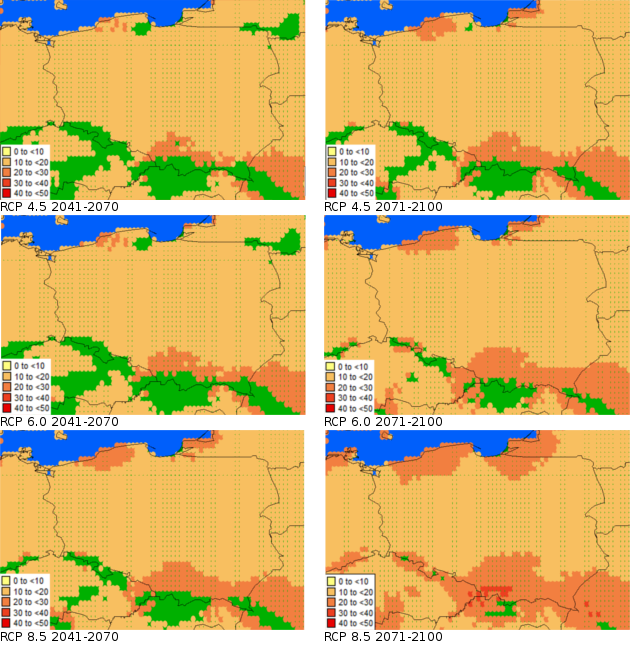
\includegraphics[width=1\linewidth]{heliothis_projekcje2} \caption{Indeks ekoklimatyczny dla H. zea w latach 2050 i 2100 na podstawie scenariuszy A1B i A2; model MIROC-H}\label{fig:heliothisp1}
\end{figure}

\begin{figure}
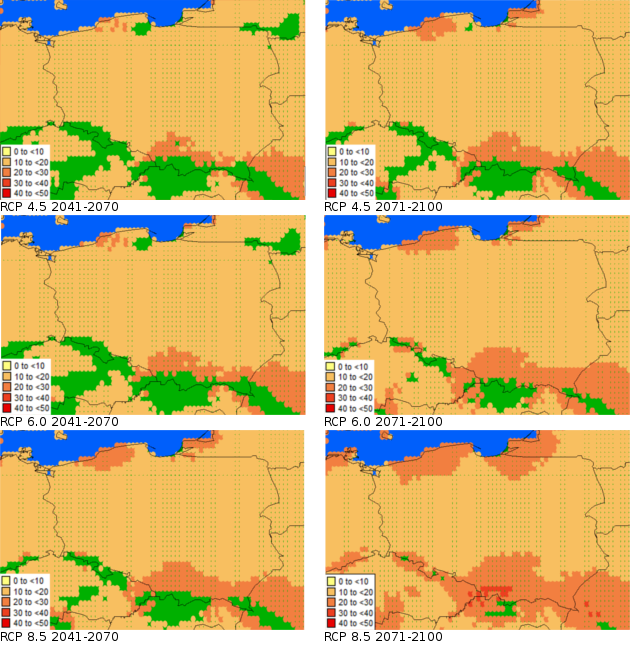
\includegraphics[width=1\linewidth]{heliothis_projekcje2} \caption{Indeks ekoklimatyczny dla H. zea w latach 2041-2070 i 2071-2100 dla scenariuszy RCP 4.5; 6.0 i 8.5}\label{fig:heliothisp2}
\end{figure}

\begin{enumerate}
\def\labelenumi{\Roman{enumi})}
\tightlist
\item
  Który scenariusz zmiany klimatu jest uwzględniony na lata 2050 do 2100
\end{enumerate}

Scenariusz zmiany klimatu: RCP 4.5, 6.0, 8.5, SRES: A2, A1B (IPCC
(\protect\hyperlink{ref-ipcc2014}{1989}))

\begin{enumerate}
\def\labelenumi{\Roman{enumi})}
\setcounter{enumi}{1}
\tightlist
\item
  Rozważyć wpływ projektowanej zmiany klimatu na agrofaga.
\end{enumerate}

Zmiany klimatyczne nie wpłyną na możliwości przenikania gatunku na
obszar PRA -- już w istniejących uwarunkowaniach klimatycznych jest ono
teoretycznie możliwe. Mogą one jednak oddziaływać na ich częstotliwość w
wypadku rozwinięcia się osiadłych populacji w pobliżu Polski (np.
północne Węgry, południe Czech). Według przyjętych modeli klimatycznych
w roku 2050 ponad połowa terytorium Polski będzie obszarem potencjalnego
zasiedlenia przez \emph{H. zea}, a w roku 2100 praktycznie cały obszar
naszego kraju (z wyjątkiem wyższych partii gór) będzie spełniał warunki
dla rozwoju tego agrofaga. Ze względu na trudność prognozowania warunków
klimatycznych w okresie zimowym, nie można w tej chwili jednoznacznie
ustalić, czy w rozpatrywanym okresie powstaną dogodne warunki do
rozwinięcia się osiadłych populacji \emph{H. zea}.

\begin{longtabu} to \linewidth {>{\raggedright\arraybackslash}p{5.5cm}>{\raggedright}X>{\raggedright\arraybackslash}p{3.5cm}}
\toprule
\rowcolor[HTML]{F5F6FA}  \textbf{Wpływ zmian klimatu na} & \textbf{Zmiana} & \textbf{Źródła}\\
\midrule
\endfirsthead
\multicolumn{3}{@{}l}{\textit{(continued)}}\\
\toprule
Wpływ zmian klimatu na & Zmiana & Źródła\\
\midrule
\endhead
\
\endfoot
\bottomrule
\endlastfoot
Czy jest prawdopodobne, że drogi przenikania mogą się zmienić na skutek zmian klimatu? & Nie & \citeauthor{eppo2018}, \hyperlink{ref-eppo2018}{\citeyear{eppo2018}}\\
Czy prawdopodobieństwo zasiedlenia może się zmienić wraz ze zmianą klimatu? & Tak; prawdopodobieństwo: średnie; niepewność: średnia & \citeauthor{kogan1989}, \hyperlink{ref-kogan1989}{\citeyear{kogan1989}}\\
Czy wielkość rozprzestrzenienia może się zmienić wraz ze zmianą klimatu? & Tak; prawdopodobieństwo: średnie; niepewność: średnia & \citeauthor{eppo2018}, \hyperlink{ref-eppo2018}{\citeyear{eppo2018}}\\
Czy wpływ na obszarze PRA może się zmienić wraz ze zmianą klimatu? & Tak; prawdopodobieństwo: średnie; niepewność: średnia & \citeauthor{eppo2018}, \hyperlink{ref-eppo2018}{\citeyear{eppo2018}}\\*
\end{longtabu}

\begin{enumerate}
\def\labelenumi{(\arabic{enumi})}
\setcounter{enumi}{15}
\tightlist
\item
  Ogólna ocena ryzyka:
\end{enumerate}

Prawdopodobieństwo zawleczenia \emph{H. zea} do Europy jest bardzo
wysokie -- w Wielkiej Brytanii wielokrotnie notowano gąsienice
przywożone wraz z importowanym materiałem roślinnym (EPPO).
Identyfikację zagrożenia ułatwia fakt, że ślady żerowania gąsienic są
zwykle dobrze widoczne i stosunkowo łatwe do wykrycia przez służby
fitosanitarne. Same larwy mogą jednak w różny sposób ukrywać się na
roślinach, między innymi wgryzając się do wnętrza łodyg, pędów, owoców
itp. Dlatego też materiał roślinny sprowadzany z obszaru występowania
agrofaga powinien być zawsze poddawany wnikliwej kontroli, a w razie
potrzeby również kwarantannie lub dezynsekcji. W naszych warunkach
dotyczy to głównie okresu wiosenno-letniego, kiedy to larwy mogłyby
dokończyć rozwój w warunkach polowych. W przypadku materiału roślinnego
sprowadzanego do uprawy w warunkach chronionych, niezbędna jest
całoroczna szczegółowa inspekcja fitosanitarna Wnikliwa inspekcja
powinna mieć także miejsce w krajach regionu śródziemnomorskiego, gdzie
gatunek ten może już obecnie zaaklimatyzować się do warunków polowych.

\part{Zarządzanie ryzykiem zagrożenia
agrofagiem.}\label{part-zarzadzanie-ryzykiem-zagrozenia-agrofagiem.}

\begin{enumerate}
\def\labelenumi{(\arabic{enumi})}
\setcounter{enumi}{16}
\tightlist
\item
  Środki fitosanitarne
\end{enumerate}

\begin{enumerate}
\def\labelenumi{\Roman{enumi})}
\tightlist
\item
  Opisać potencjalne środki dla odpowiednich dróg przenikania i ich
  oczekiwaną efektywność na zapobieganie wprowadzenia (wejście i
  zasiedlenie) oraz/lub na rozprzestrzenienie.
\end{enumerate}

\begin{longtabu} to \linewidth {>{\raggedright}X>{\raggedright\arraybackslash}p{4.5cm}>{\raggedright\arraybackslash}p{4.5cm}}
\toprule
\rowcolor[HTML]{F5F6FA}  \textbf{Możliwe drogi przenikania (w kolejności od najważniejszej)} & \textbf{Możliwe środki} & \textbf{Opłacalność środków}\\
\midrule
\endfirsthead
\multicolumn{3}{@{}l}{\textit{(continued)}}\\
\toprule
Możliwe drogi przenikania (w kolejności od najważniejszej) & Możliwe środki & Opłacalność środków\\
\midrule
\endhead
\
\endfoot
\bottomrule
\endlastfoot
Transport lotniczy całych roślin lub ich części. & Wykrycie w przesyłkach poprzez inspekcję przed odprawą lub trakcie transportu. & Wysoka\\
Transport lotniczy całych roślin lub ich części. & Wykrycie podczas kwarantanny po wejściu. & Średnia\\
Transport lotniczy całych roślin lub ich części. & Eradykacja z użyciem insektycydów. & Wysoka opłacalność, niskie koszty insektycydów.\\*
\end{longtabu}

\begin{enumerate}
\def\labelenumi{\Roman{enumi})}
\setcounter{enumi}{1}
\tightlist
\item
  Środki zarządzania eradykacją, powstrzymywaniem i kontrolą
\end{enumerate}

Podstawową metodą zapobiegania wniknięcia agrofaga jest wnikliwa
kontrola fitosanitarna, która może odbywać się na różnych etapach
transportu -- od momentu przygotowywania roślin (lub ich części) po
rozładunek w miejscu docelowym. Szczególnie istotne jest to w miesiącach
wiosenno-letnich, kiedy to gąsienice mogłyby dokończyć swój rozwój w
warunkach polowych, a jako polifag, dość łatwo znajduje rośliny
pokarmowe. W wypadku wątpliwości co do zainfekowania sprowadzanego
materiału, należy go poddać kwarantannie. Jeśli charakter materiału na
to pozwala (np. nie są to rośliny przeznaczone do konsumpcji), powinny
zostać wykonane zabiegi z użyciem środków ochrony roślin o szerokim
spektrum działania (np. chloropiryfos). Można również stosować
schładzanie materiału przez 2-4 dni w temperaturze 1.7°C a następnie
fumigację bromkiem metylu w dawce 13.5 g/m3 przez 4 godziny. Rośliny
przeznaczone do konsumpcji, których dezynsekcja jest niemożliwa, powinny
zostać zniszczone, np. przez spalenie.

\begin{enumerate}
\def\labelenumi{(\arabic{enumi})}
\setcounter{enumi}{17}
\tightlist
\item
  Niepewność:
\end{enumerate}

Brak dostępnych informacji o przypadkach stwierdzenia na obszarze PRA
przypadków odnalezienia \emph{H. zea} w importowanym materiale
roślinnym. W wypadku bardzo małych larw lub złóż jaj, możliwe jest ich
przeoczenie przez służby fitosanitarne. W razie uzasadnionych podejrzeń
sprowadzony materiał należy poddać kwarantannie.

\begin{enumerate}
\def\labelenumi{(\arabic{enumi})}
\setcounter{enumi}{18}
\tightlist
\item
  Uwagi:
\end{enumerate}

W obecnych warunkach klimatycznych środki fitosanitarne nie są konieczne
w miesiącach zimowych, gdyż gatunek ten nie jest wstanie przetrwać w
warunkach polowych. Nie dotyczy to jednak roślin sprowadzanych do
dalszej uprawy w warunkach chronionych.

Występowanie w Europie bliźniaczego gatunku H. armigera, komplikuje
nieco status \emph{H. zea}. Rozróżnienie ich w stadium gąsienicy jest
prawie niemożliwe, a identyfikacja na podstawie postaci dorosłych wymaga
specjalistycznej wiedzy. Paradoksalnie występowanie \emph{H. armigera}
może utrudniać wniknięcie \emph{H. zea}, gdyż zajmują podobne nisze
ekologiczne.

\appendix


\section{Zdjęcia}\label{zdjecia}

\section{Klimat}\label{klimat}

Modele i warunki klimatyczne.

\begin{longtabu} to \linewidth {>{\raggedright\arraybackslash}p{4.5cm}>{\raggedright\arraybackslash}p{1.5cm}>{\raggedright}X>{\raggedleft\arraybackslash}p{1.5cm}}
\toprule
\rowcolor[HTML]{F5F6FA}  \textbf{Czynnik klimatyczny} & \textbf{kod} & \textbf{opis} & \textbf{wartość}\\
\midrule
\endfirsthead
\multicolumn{4}{@{}l}{\textit{(continued)}}\\
\toprule
Czynnik klimatyczny & kod & opis & wartość\\
\midrule
\endhead
\
\endfoot
\bottomrule
\endlastfoot
 & DV0 & temperatura limitująca dolna & 12.0000\\

 & DV1 & temperatura optymalna dolna & 18.0000\\

 & DV2 & temperatura optymalna gótna & 35.0000\\

\multirow{-4}{4.5cm}{\raggedright\arraybackslash Temperatura} & DV3 & temperatura limitująca górna & 42.0000\\
\cmidrule{1-4}
 & SM0 & wilgotność limitująca dolna & 0.0200\\

 & SM1 & wilgotność optymalna dolna & 0.7000\\

 & SM2 & wilgotność optymalna górna & 1.5000\\

\multirow{-4}{4.5cm}{\raggedright\arraybackslash Wilgotność} & SM3 & wilgotność limitująca górna & 2.5000\\
\cmidrule{1-4}
 & DPD0 & Długość dnia inicjująca diapuazę & 12.0000\\

 & DPT0 & Temperatura inicjująca diapauzę & 12.0000\\

 & DPT1 & Temperatura hamująca diapauzę & 13.0000\\

 & DPD0 & Liczba dnia potrzebna do ukończenia diapauzy & -69.0000\\

\multirow{-5}{4.5cm}{\raggedright\arraybackslash Diapauza} & DPSW & Wskaźnik: 0 – diapauza zimowa, 1 – diapauza letnia & 0.0000\\
\cmidrule{1-4}
 & TTCS & temperatura progowa & 5.0000\\

\multirow{-2}{4.5cm}{\raggedright\arraybackslash Stres zimna} & THCS & tempo akumulacji & -0.0003\\
\cmidrule{1-4}
 & TTHS & temperatura progowa & 42.0000\\

\multirow{-2}{4.5cm}{\raggedright\arraybackslash Stres cieplny} & THHS & tempo akumulacji & 0.0010\\
\cmidrule{1-4}
 & SMDS & wilgotność progowa & 0.0200\\

\multirow{-2}{4.5cm}{\raggedright\arraybackslash Stres suszy} & HDS & tempo akumulacji & -0.0050\\
\cmidrule{1-4}
 & SMWS & wilgotność progowa & 2.5000\\

\multirow{-2}{4.5cm}{\raggedright\arraybackslash Stres wilgotności} & HWS & tempo akumulacji & 0.0050\\
\cmidrule{1-4}
 & DTCW & Minimalna liczba stopniodni powyżej DVCS & 80.0000\\

 & MTCW & wilgotność progowa & 1.0000\\

\multirow{-3}{4.5cm}{\raggedright\arraybackslash Stres zimna-wilgotności} & PCW & tempo akumulacji & 0.1000\\
\cmidrule{1-4}
 & DV0 &  & 12.0000\\

\multirow{-2}{4.5cm}{\raggedright\arraybackslash Akumulacja stopnio-dni powyżej DV0} & DV3 &  & 42.0000\\
\cmidrule{1-4}
 & DV3 &  & 42.0000\\

\multirow{-2}{4.5cm}{\raggedright\arraybackslash Akumulacja stopnio-dni powyżej DV3} & DV4 &  & 100.0000\\
\cmidrule{1-4}
 & DVCS &  & 0.0000\\

\multirow{-2}{4.5cm}{\raggedright\arraybackslash Akumulacja stopnio-dni powyżej DVCS} & DV4 &  & 100.0000\\
\cmidrule{1-4}
Stoopnio-dni na pokolenie & PDD & minimalna liczna stopnio-dni powyżej DV0 do ukończenia pokolenia & 690.0000\\*
\end{longtabu}

\section*{Źródła}\label{zroda}
\addcontentsline{toc}{section}{Źródła}

\hypertarget{refs}{}
\hypertarget{ref-billen1984}{}
Billen, W., 1984. Tropische Insekten in Basel. Mitteilungen der
Entomologischen Gesellschaft Basel 34, 141--144.

\hypertarget{ref-cabi2017}{}
CABI, 2018. textitHelicoverpa zea {[}WWW Document{]}. URL
\url{https://www.cabi.org/isc/datasheet/26776} (udostępniono 9.28.18).

\hypertarget{ref-cabieppo2017}{}
CABI/EPPO, 2017. EPPO quarantine pest Prepared by CABI and EPPO for the
EU under Contract 90/399003 Data Sheets on Quarantine Pests Helicoverpa
zea {[}WWW Document{]}. URL
\url{https://extension.entm.purdue.edu/CAPS/pdf/datasheets/OldWorldBollworm.pdf}
(udostępniono 9.28.18).

\hypertarget{ref-capinera2000}{}
Capinera, J., 2000. Corn Earworm, textitHelicoverpa (=Heliothis) zea
(Boddie) (Lepidoptera: Noctuidae) Florida Cooperative Extension Service
{[}WWW Document{]}. URL
\url{http://entnemdept.ufl.edu/creatures/veg/corn_earworm.htm}
(udostępniono 9.28.18).

\hypertarget{ref-csiro2004}{}
Commonwealth Scientific and Industrial Research Organisation (CSIRO),
2004. Dymex Simulator Application 2.0. Hearn Scientific Software,
Australia.

\hypertarget{ref-eppo2018}{}
EPPO, 2018. EPPO Global Database (available online) {[}WWW Document{]}.
URL \url{https://gd.eppo.int} (udostępniono 9.28.18).

\hypertarget{ref-ipcc2014}{}
IPCC, 1989. Summary for policymakers, w: Field, C., Barros, V., Dokken,
D., al. (Red.), Climate Change 2014: Impacts, Adaptation, and
Vulnerability. Part A: Global and Sectoral Aspects. Contribution of
Working Group II to the Fifth Assessment Report of the Intergovernmental
Panel on Climate Change. Cambridge University Press, Cambridge, United
Kingdom; New York, USA, ss. 1--32.

\hypertarget{ref-kogan1989}{}
Kogan, M., Helm, C., Kogan, J., Brewer, E., 1989. Distribution and
economic importance of Heliothis virescens and textitHelicoverpa zea in
North, Central, and South America and of their natural enemies and host
plants., w: King, E., Jackson, R. (Red.), Proceedings of the workshop on
the biological control of Heliothis: increasing the effectiveness of
natural enemies. USDA, Far East Regional Office, New Delhi, Indie, ss.
241--297.

\hypertarget{ref-kriticos2012}{}
Kriticos, D., Webber, B., Leriche, A., Ota, N., Macadam, I., Bathols,
J., Scott, J., 2012. CliMond: global high resolution historical and
future scenario climate surfaces for bioclimatic modelling. Methods in
Ecology and Evolution 3, 53--64.

\hypertarget{ref-lepintercept2017}{}
Lepintercept, 2017. Lepintercept. An identification resource for
intercepted Lepidoptera larvae {[}WWW Document{]}. URL
\url{http://idtools.org/id/leps/lepintercept/zea.html} (udostępniono
9.28.18).

\hypertarget{ref-mika2010}{}
Mika, A., Newman, J., 2010. Climate change scenarios and models yield
conflicting predictions about the future risk of an invasice species in
North America. Agricultural and Forest Entomology 12, 213--221.

\hypertarget{ref-olmstead2016}{}
Olmstead, D., Nault, B., Shelton, A., 2016. Biology, ecology, and
evolving management of Helicoverpa zea (Lepidoptera: Noctuidae) in sweet
corn in the United States. Journal of Economic Entomology Advance 109,
1667--1676.

\hypertarget{ref-passoa2014}{}
Passoa, S., 2014. Key to the identification of Helicoverpa armigera
suspects intercepted at U.S. ports of entry, w: Gilligan, T., Passoa,
S.C. (Red.), LepIntercept, An identification resource for intercepted
Lepidoptera larvae. USDA/APHIS/PPQ/S\&T, Fort Collins, CO., USA, ss.
1--3.

\hypertarget{ref-purcell1992}{}
Purcell, M., Johnson, M.W., Lebeck, L.M., Hara, A.H., 1992. Biological
control of Helicoverpa zea (Lepidoptera: Noctuidae) with Steinernema
carpocapsae (Rhabditida: Steinernematidae) in corn used as a trap crop.
Environmental Entomology 21, 1441--1447.

\hypertarget{ref-rcore2018}{}
R Core Team, 2018. R: A Language and Environment for Statistical
Computing. R Foundation for Statistical Computing, Vienna, Austria.

\hypertarget{ref-xie2016}{}
Xie, Y., 2016. bookdown: Authoring Books and Technical Documents with R
Markdown. Chapman; Hall/CRC, Boca Raton, Florida.

\hypertarget{ref-xie2015}{}
Xie, Y., 2015. Dynamic Documents with R and knitr, 2nd ed. Chapman;
Hall/CRC, Boca Raton, Florida.

\hypertarget{ref-luliang2002}{}
YongYue, L., GuangWen, L., 2017. Spatial pattern of cotton bollworm
(Helicoverpa zea) eggs with geostatistics. Journal of Huazhong
Agricultural University 21, 13--17.

\hypertarget{ref-zalucki2005}{}
Zalucki, M., Furlong, M., 2015. Forecasting Helicoverpa populations in
Australia: A comparison of regression based models and a bio-climatic
based model approach. Insect Science 12, 45--56.


\end{document}
